\documentclass[UTF8]{ctexart}
\usepackage{amsmath,graphicx,tikz,caption,subfigure}
\usepackage[algo2e,ruled,vlined]{algorithm2e}
\usepackage{stfloats}
\usepackage{float}
\usepackage[a4paper]{geometry}
\geometry{left=0.5cm,right=0.5cm,top=0.5cm,bottom=0.5cm}
\title{\textbf{Report4}}
\author{PB21000235 胡琦浩}
\date{\today}

\begin{document}
\maketitle
\section{问题}
设pdf函数满足关系式:
\begin{equation}
    p'(x)=a\delta (x)+b\cdot exp(-cx)
\end{equation}
讨论该函数性质并给出抽样方法。

\section{方法}
\subsection{数学推导}
\subsubsection{$c=0$且$b\neq 0$}
$p'(x)=a\delta (x)+b$,\quad 积分可得:$p(x)=aH(x)+bx+A$,式中$A$为积分常数.

由于$p(x)$满足归一化,则:
\begin{equation}
    \int_{-1}^{1} p(x) \,dx = \int_{-1}^{1} (aH(x)+bx+A) \,dx=a+2A=1  
\end{equation}

简洁起见,令$a=1$,则$A=0$.\quad 故$p(x)=H(x)+bx$

由于$p(x)$非负,则$b\in [-1,0)$

求累计函数:
\begin{equation}
    \xi(x)=\int_{-1}^{x} p(t) \,dt =xH(x)+\frac{1}{2}b(x^2-1)\in[0,1]
\end{equation}

变化可得:
\begin{equation}
    bx^2+2xH(x)-(b+2\xi )=0
\end{equation}

当$x\in [0,1]$时,$H(x)=1$,此时:
\begin{equation}
    \Delta =4+4b(b+2)\geq 0
\end{equation}
恒成立

解得:
\begin{equation}
    x_1=\frac{-1+\sqrt{1+b(b+2\xi )}}{b}
\end{equation}
\begin{equation}
    x_2=\frac{-1-\sqrt{1+b(b+2\xi) }}{b}
\end{equation}

要满足约束条件,则$\xi \in [-\frac{b}{2},1]$时,$x_1$为此方程的解

当$x\in [-1,0)$时,$H(x)=0$,此时:
\begin{equation}
    bx^2-(b+2\xi)=0
\end{equation}

解得:
\begin{equation}
    x_3=\sqrt{\frac{b+2\xi}{b}}
\end{equation}
\begin{equation}
    x_4=-\sqrt{\frac{b+2\xi}{b}}
\end{equation}

要满足约束条件,则$\xi \in[0,-\frac{b}{2})$时,$x_4$为此方程的解

综上所述(令$b=-1$,此时$p(x)=H(x)-x$):

当$\xi \in[0,\frac{1}{2})$时,$x=-\sqrt{1-2\xi}$

当$\xi \in [\frac{1}{2},1]$时,$x=1-\sqrt{2-2\xi}$

\subsubsection{$b=0$}
依据前面的假定,易得:$p'(x)=\delta (x)$,\quad $p(x)=H(x)$,\quad $\xi(x)=xH(x)$

当$\xi=0$时,$x\in[-1,0]$

当$\xi\in(0,1]$时,$x=\xi$

\subsubsection{$bc\neq 0$}
积分可得:$p(x)=aH(x)-\frac{b}{c}e^{-cx}+A$,$A$为积分常数

由归一化条件可得:
\begin{equation}
    \int_{-1}^{1} p(x) \,dx =a+\frac{b}{c^2}(e^{-c}-e^c)+2A=1
\end{equation}

考虑到$x\in[-1,1]$时,$p(x)\geq0$恒成立
,故令$a=e^\frac{1}{3}+1-3e^{-\frac{1}{3}}=0.246,b=c=\frac{1}{3}$,计算可得:$A=e^{\frac{1}{3}}$

故:$p(x)=0.246H(x)-e^{-\frac{x}{3}}+e^{\frac{1}{3}}$

由于较难求出反函数,故使用舍选法:

显然$p(x)$是一个单调递增的函数,故$M=p(1)=2e^\frac{1}{3}+1-4e^{-\frac{1}{3}}=0.925$

由简单分布的公式:令$x=2\xi_1-1$,\quad $y=M\xi_2$

当$M\xi_2\leq p(2\xi_1-1)$时,取$x=2\xi_1-1$.否则重新选取$(\xi_1,\xi_2)$

\subsection{代码实现}
\subsubsection{$c=0$且$b\neq 0$}
先利用Schrage方法生成100000个随机数储存到$\xi$,然后根据公式(6)与(10)得出$\xi$.然后作概率直方图与理论p(x)进行比较

\subsubsection{$b=0$}
同2.2.1的方法

\subsubsection{$bc\neq 0$}
先生成2000000个随机数,前1000000个赋给$\xi_1$,后1000000个赋给$\xi_2$

然后根据2.1.3中的舍选法得到样本x即可,最后作图检验

\section{实验结果}
\begin{figure}[H]
    \centering
    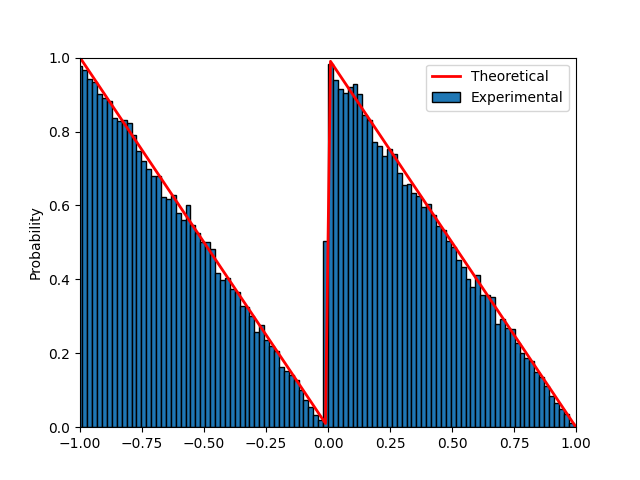
\includegraphics[scale=0.5]{1.png}
    \caption{$c=0$且$b\neq 0$,样本数$N=100000$}
\end{figure}
\begin{figure}[H]
    \centering
    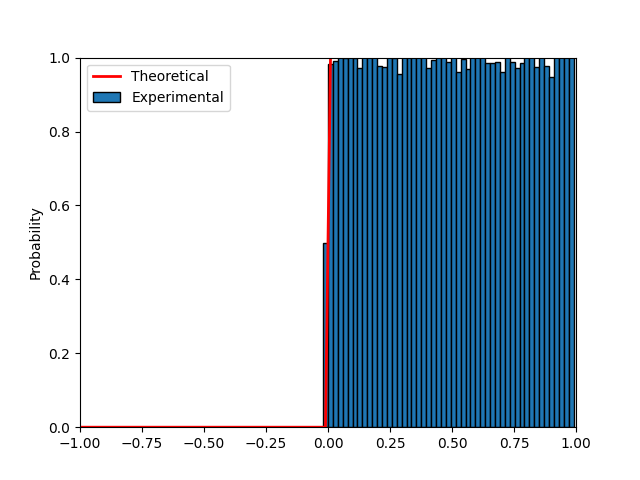
\includegraphics[scale=0.5]{2.png}
    \caption{$b=0$,样本数$N=100000$}
\end{figure}
\begin{figure}[H]
    \centering
    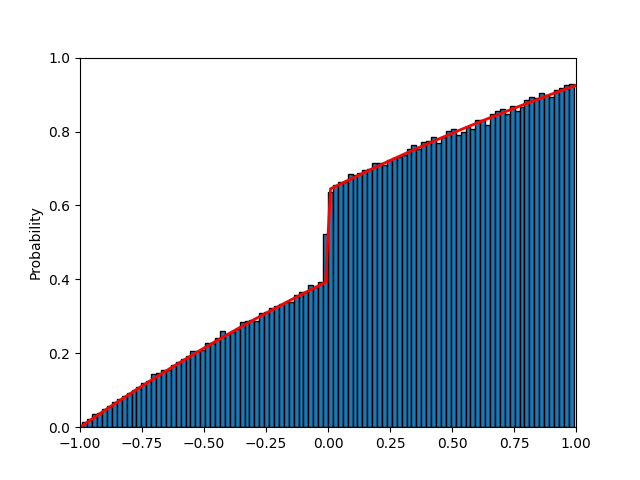
\includegraphics[scale=0.5]{3.png}
    \caption{$bc\neq 0$,样本数$N=540973$}
\end{figure}

可以看出,前两种用直接抽样法与理论函数符合的很好,后面一种用舍选法也与理论函数符合的很好
\section{总结}
该实验让我熟悉了概率函数密度的性质,并加深了对舍选法的了解
\end{document}